\section{Data translation}
\subsection{Data collection}
In order to collect suitable data we tried different data service providers such as Datahub, finally we have collected total four datasets from three different sources and in three different formats, including: 

%For each subsubsection below:
%Which format did the data have? CSV, JSON, XLSX?
%Size of each dataset? (how many entities)
%Which attributes were collected for each dataset? 
%Why? Optional ones? Nonoptional ones? Resulting sparsity of each attribute?
%How did collect each dataset? Queries (give an excerpt), downloads...




\subsubsection{Forbes: Company}
%Silvia/Zehui
The Forbes offers a .xls file with a list of Top 2000 companies during the period 2000 to 2014 which were published in Forbes magazine because of great performance in terms of business achievements. This dataset describes the basic information about these top 2000 companies. For example, location shows where this company is founded, industry depicts what fields the company focus on and so on.
\subsubsection{DBpedia: Company }
The information of company is extracted from DBpedia, since it provides relatively complete information.  To access information from DBPedia we used the public SPARQL endpoint (at http://dbpedia.org/sparql). Figure 1.1 is our query for company, actually there is total 764398 companies in DBpedia, which would be too much for us and also not easy to handle it in terms of processing time and space. In order to reduce the number of data, we limit the company types to "company" and "public company" and only extract the companies that provide attributes "LocationCity" and "LocationCountry", these two attributes can also be related with Location Information, that's why we consider them as necessary and others are optional. On the other hand, if all these attributes are necessary, there will be only few thousands companies extracted, because not all companies have all these nine attributes, in this case few overlapping data will be in the final integration results. In addition to this, as many attributes such as KeyPeople, locationCity have multiple values which result in the same company would appear more than one times, to avoid these duplicates we used "group\_contac", a function in Sparql, to group many value together. There are also many values for Revenue but without date notation, so we just took the maximum value. 

%\begin{figure}[H]
%	\begin{center}
%	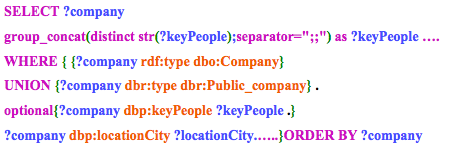
\includegraphics[width=10cm]{DB_Com}
%	\caption[DBpedia Query For Company]{DBpedia Query For Company}
%	\label{fig:db}
%	\end{center}
%\end{figure}

\subsubsection{Freebase: Company}
%Yiru
Freebase provides web service to query data and return in JSON. The total number of entities is 3,182. We make name nonoptional, since we want to use it to compare companies in each dataset. Also, number\_of\_employees is nonoptional, because the amount for being optional is around 230,000 and we don't want to use it. The rest attributes are all optional.
First we test queries on the query page to make sure we get the right data. Then, we build a Java project to execute the MQL Read API which provides access to the Freebase database by Metaweb query language (MQL). Additionally, during the mapping procedure, we occur some problem about multiple values in JSON array and JSON object, it couldn't match in target schema because of the various number of values. Thus, we convert them into one string and separate with two semicolons while excuting Java project.


\subsubsection{DBpedia: Location}
%Silvia/Zehui
We also extracted Location information from DBpedia with the same method as Company. Figure 1.2 is the query for location. For the same reason as Company, we limit the location types to "city" and "AdministrativeRegion", which are more relevant to our company dataset. Also some attributes have many values without extra information, it's hard to identify which one represents the current state, thus, we just took the maximum number of them among multiple values. Furthermore, the name of locations are provide in different languages, while in our project we just focus on english, so we filtered language as english.

%\begin{figure}[H]
%	\begin{center}
%	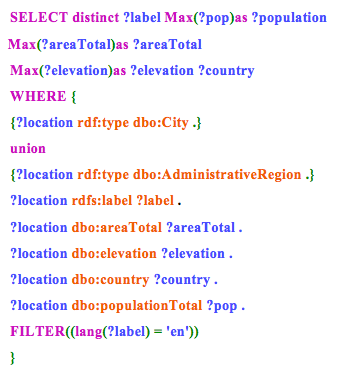
\includegraphics[width=10cm]{DB_Loc}
%	\caption[DBpedia Query For Location]{DBpedia Query For Location}
%	\label{fig:db}
%	\end{center}
%\end{figure}


\begin{table}[H]
\centering
\begin{tabular}{|l|l|l|l|l|l|}
\hline
 & Source & Format & Class & \#Entities & \#Attributes \\ \hline
 & \multicolumn{5}{c|}{List of attributes} \\ \hline
\multirow{2}{*}{Forbes} & forbes.com & xlsx & company & \multicolumn{1}{c|}{2000} & \multicolumn{1}{c|}{7} \\ \cline{2-6} 
 & \multicolumn{5}{l|}{\begin{tabular}[c]{@{}l@{}}name, countries, industries, revenue, assets,\\ marketValue, profit\end{tabular}} \\ \hline
\multirow{2}{*}{DBpedia} & dbpedia.org/sparql & csv & company & \multicolumn{1}{c|}{16051} & \multicolumn{1}{c|}{9} \\ \cline{2-6} 
 & \multicolumn{5}{l|}{\begin{tabular}[c]{@{}l@{}}name, countries, industries, revenue, numberOfEmployees,\\ dateFounded, profit, keyPeople, locations\end{tabular}} \\ \hline
\multirow{2}{*}{Freebase} & freebase.com/query & json & company & 3182 & 9 \\ \cline{2-6} 
 & \multicolumn{5}{l|}{\begin{tabular}[c]{@{}l@{}}name, countries, industries, revenue, numberOfEmployees,\\ dateFounded, profit, keyPeople, locations\end{tabular}} \\ \hline
\multirow{2}{*}{DBpedia} & dbpedia.org/sparql & csv & location & 3270 & 5 \\ \cline{2-6} 
 & \multicolumn{5}{l|}{locationName, country, population, area, elevation} \\ \hline
\end{tabular}
\caption{Basic profile of each dataset}
\label{my-label}
\end{table}




\subsection{Integrated schema}
%Take from data\ForbesPlan\Forbes-integrated schema.docx
We looked into four datasets and did the following Integrated Schema.In this table we use prefix dataset 1, 2, 3,4 respectively represent Forbes, DBpedia(company), Freebase and DBpedia(Location)

%================ BEGIN TABLE

\begin{table}[H]
\centering
\begin{tabular}{|c|c|c|}
\hline
\textbf{Class Name} & \textbf{Attributes Name} & \textbf{\begin{tabular}[c]{@{}c@{}}Datasets in which\\ the attribute is found\end{tabular}} \\ \hline
company & (company) name & dataset 1, 2, 3 \\ \hline
company, location & country & dataset 1, 2, 3, 4 \\ \hline
company & industries & dataset 1, 2, 3 \\ \hline
company & revenue & dataset 1, 2, 3 \\ \hline
company & numberOfEmployees & dataset 2, 3 \\ \hline
company & dateFounded & dataset 2, 3 \\ \hline
company & assets & dataset 1, 2 \\ \hline
company & marketValue & dataset 1 \\ \hline
company & profit & dataset 1, 3 \\ \hline
company & continent & dataset 1 \\ \hline
company & keyPeople & dataset 2, 3 \\ \hline
company, location & (location) name & dataset 2, 3, 4 \\ \hline
location & population & dataset 4 \\ \hline
location & area & dataset 4 \\ \hline
location & elevation & dataset 4 \\ \hline
\end{tabular}
\caption{Integrated schema}
\label{my-label}
\end{table}

%==================== END TABLE




\subsection{Data transformations}
Transformations were applied at two different points in this phase. The first was applied during mapping while the second was applied in the Java project. To begin with, numeric attributes with big values such as revenue or assets were often retrieved in scientific notation. Accordingly a function within MapForce was used to convert the numbers into a decimal notation. Secondly the datasets did not possess an ID attribute. Because it was going to be used later, it was generated with "GenerateID" in MapForce. 

The next transformations occured in Java. Many values, especially from the two DBpedia datasets, were loaded in the form of a URL due to our SPARQL query. As such the URL was parsed and only the actual value was kept. In addition, punctation and symbols such as "\_" were removed. Lastly we normalized country values, which was an important step for the blocking functions used later on in identity resolution. Especially values for the USA were transformed from spellings such as "US", "USA", "United States" to "United States of America".



%Numeric attributes to do with money: Scientific notation, small values from Forbes
%	e.g. 1.17E+10 ==> 11.700.000.000
% 	e.g. 483,1 (Apple in Forbes) ==> 483.100.000.000
%DBpedia values: Very often URL
%Company and location names: Removed common strings that are inconsistent among datasets, e.g. Apple / Apple, Inc.
% 	also: Replaced punctuation and symbols like "_" or "."
%	Result example: Apple (Forbes) <-> Apple,_Inc (DBpedia)


%Oliver
%Which attributes did we transform in which way? 
%Also: Example for each transformation showing why we did it


%Countries: Replaced different spellings of same word 
%	e.g. US, USA, U.S., America with "United States of America" or UK, England with United Kingdom


%=================================== OLD
%\begin{table}[H]
%\centering
%\caption{Integrated Schema}
%\label{my-label}
%\begin{tabular}{|c|c|c|c|}
%\hline
%Class Name & Attributes Name & \begin{tabular}[c]{@{}c@{}}Datasets in which \\ attribute is found\end{tabular} & \begin{tabular}[c]{@{}c@{}}Conflict resolution\\        %strategies\end{tabular} \\ \hline
%company & (company)name & dataset 1, 2, 3 & \begin{tabular}[c]{@{}c@{}}LongestString, \\ FavourSources, \\ Voting\end{tabular} \\ \hline
%company,location & country & dataset 1, 2, 3, 4 & Voting \\ \hline
%company & industries & dataset 1, 2, 3 & Union \\ \hline
%company & \begin{tabular}[c]{@{}c@{}}Sales/\\ revenue\end{tabular} & dataset 1, 2, 3 & FavourSources \\ \hline
%company & \begin{tabular}[c]{@{}c@{}}number Of \\ Employees\end{tabular} & dataset 2, 3 & \begin{tabular}[c]{@{}c@{}}Average,\\ Growth: Max\end{tabular} \\ \hline
%company & \begin{tabular}[c]{@{}c@{}}founding year/ \\ date founded\end{tabular} & dataset 2, 3 & \begin{tabular}[c]{@{}c@{}}MostComplete\\ (complete date) \\ AND,\\ MostComplete \\ %(sample)\end{tabular} \\ \hline
%company & Assets & dataset 1, 2 & FavourSources \\ \hline
%company & Market Value & dataset 1 & / \\ \hline
%company & profit & dataset 1, 3 & FavourSources \\ \hline
%company & continent & dataset 1 & / \\ \hline
%company & \begin{tabular}[c]{@{}c@{}}keyPeople/\\  leadership\end{tabular} & dataset 2, 3 & Union \\ \hline
%\begin{tabular}[c]{@{}c@{}}company,\\ location\end{tabular} & name & dataset 2, 3, 4 & \begin{tabular}[c]{@{}c@{}}Union AND \\ FavourSources\end{tabular} \\ \hline
%location & \begin{tabular}[c]{@{}c@{}}population\\ total\end{tabular} & dataset 4 & / \\ \hline
%location & area total & dataset 4 & / \\ \hline
%location & elevation & dataset 4 & / \\ \hline
%\end{tabular}
%\end{table}


